\documentclass[sigconf,authorversion,nonacm]{acmart}

%%% ADDED PACKAGES %%%
\usepackage{url}
\usepackage[belowskip=0pt,aboveskip=5pt]{subcaption}
\usepackage{listings}
\usepackage{enumitem}
\usepackage{booktabs}
\usepackage{xspace}
\usepackage{makecell}
\usepackage{amsmath}
\usepackage{pifont}
\usepackage{balance}
\usepackage{soul}
\usepackage{microtype}    
\usepackage[ruled,vlined,linesnumbered]{algorithm2e}
\usepackage[noend]{algpseudocode}
\usepackage{amsthm}
\usepackage{comment}
\usepackage{xr}
\usepackage{color}
\usepackage{setspace}
\usepackage{listings}
\usepackage{lipsum}
\usepackage{adjustbox}
\usepackage{array,multirow,graphicx}
\usepackage{float}
\usepackage{graphicx}

\lstdefinestyle{code}{
  backgroundcolor=\color{gray!4},
  commentstyle=\color{codegray},
  keywordstyle=\color{codepurple},
  numberstyle=\tiny\color{codegray},
  stringstyle=\color{codegray},
  basicstyle=\ttfamily\footnotesize,
  breakatwhitespace=false,         
  breaklines=true,                 
  captionpos=b,                    
  keepspaces=true,                 
  numbers=left,                    
  numbersep=5pt,                  
  showspaces=false,                
  showstringspaces=false,
  showtabs=false,                  
  tabsize=2,
  % escapeinside=||
}
\lstset{style=code}

\lstset{escapeinside={<@}{@>}}
%%% ADDED Commands %%%
\definecolor{comment}{rgb}{0,0.6,0}
\definecolor{dgray}{gray}{0.25}
\definecolor{strings}{RGB}{0,0,128}
\definecolor{backcolour}{rgb}{0.95,0.95,0.92}
\definecolor{keywords}{RGB}{127,0,85}
\definecolor{darkred}{RGB}{139,0,0}
\definecolor{darkyellow}{RGB}{204,204,0}
\definecolor{darkblue}{rgb}{0.0, 0.0, 0.55}
\definecolor{vividviolet}{rgb}{0.62, 0.0, 1.0}
\definecolor{fuchsia}{rgb}{1.0, 0.0, 1.0}
\definecolor{shockingpink}{rgb}{0.99, 0.06, 0.75}
\definecolor{darkBlue}{RGB}{0, 0, 205}
\lstset{breaklines=true}
\captionsetup[lstlisting]{font={tiny}}
\definecolor{problemblue}{RGB}{100,134,158}
\definecolor{idiomsgreen}{RGB}{0,162,0}
\definecolor{exercisebgblue}{rgb}{0,  .69,  .941}
\definecolor{deepgreen}{rgb}{0.0, 0.5, 0.0}
\definecolor{codegreen}{rgb}{0,0.6,0}
\definecolor{codegray}{rgb}{0.5,0.5,0.5}
\definecolor{codepurple}{rgb}{0.58,0,0.82}
\definecolor{backcolour}{rgb}{0.95,0.95,0.92}
\definecolor{redColor}{RGB}{255,0,0}
\definecolor{Gray}{gray}{0.1}
\definecolor{CadetBlue}{RGB}{243.0,42.1,134.0}

%%% Packages for Algorithms %%%
\usepackage[linesnumbered,ruled,vlined]{algorithm2e}
\SetKwInput{KwInput}{Input}                % Set the Input
\SetKwInput{KwInputs}{Inputs}                % Set the Input
\SetKwInput{KwOutput}{Output}              % set the Output

\begin{document}

\title{CS 537 Research Project Proposal}

\author{Aman Jain}
\affiliation{
    \institution{University of Illinois at Urbana-Champaign}
}
\email{aman18@illinois.edu}

\begin{abstract}
IoT dashboards increasingly depend on continuous, high-rate sensor streams, but naïvely forwarding every update end-to-end can overwhelm bandwidth, inflate tail latency, and yield unstable displays when the last hop degrades (loss, jitter, bandwidth caps, or short outages). Existing edge and gateway reduction techniques often reduce traffic volume, yet they do not consistently make dashboard-oriented semantics first-class—particularly under MQTT reliability settings where QoS~1 provides ``at least once'' delivery and duplicates may occur, complicating correctness and increasing overhead \cite{mqtt311}. We propose \textit{Agrasandhani}, an MQTT-based smart gateway that cleans and summarizes sensor streams via hybrid time/size batching, message-ID deduplication, within-batch latest-per-sensor compaction, and adaptive publish-rate control based on publish health signals, coupled with last-known-good dashboard semantics that expose an explicit freshness (age) indicator with a TTL. We will evaluate an ablation ladder of gateway variants (V0--V4) under QoS~0 and QoS~1 using deterministic, repeatable network impairments (bandwidth caps, loss, delay/jitter, and outages) injected primarily on the gateway-to-dashboard path with Linux traffic control (e.g., \texttt{tc netem}) \cite{jurgelionis2011_netem_empirical}, reporting end-to-end latency (including p95/p99), message rate, bandwidth usage, data loss, and freshness to characterize the trade-offs between communication reduction, timeliness, and user-visible stability.
\end{abstract}

\maketitle

\section{Artifact Information}

Link to the GitHub Repository: \\
https://github.com/AJMSD/Agrasandhani

\section{Introduction}

% [proposal] Importance of the problem
IoT deployments increasingly rely on continuous, high-rate sensor streams to drive real-time dashboards and automation. However, under bursty workloads and imperfect networks, naïvely forwarding every sensor message to the UI can overwhelm bandwidth, inflate end-to-end latency, and produce unstable or misleading displays (e.g., rapid flicker, gaps, or apparent “randomness” when updates arrive late or out of order). This is especially problematic for human-facing monitoring, where the user’s experience depends not just on whether messages eventually arrive, but on whether the displayed state remains timely, interpretable, and stable under loss, jitter, and temporary outages. Motivated by these constraints, our project studies an MQTT-based IoT gateway that can reduce communication overhead while preserving actionable dashboard behavior when network conditions degrade.

% [proposal] State of the art techniques (1/2)
A common direction in the literature is to reduce IoT communication cost by moving computation closer to the edge/fog layer: gateways and edge services filter redundant updates, aggregate multiple readings, compress payloads, or adapt sampling rates to lower network and storage pressure. Systematic reviews and mappings of edge/fog data reduction techniques emphasize that aggregation and filtering (including window-based summarization and suppression of redundant updates) are among the most frequently explored strategies because they are practical, protocol-agnostic, and provide direct reductions in transmitted volume. These approaches typically target trade-offs between data fidelity and resource usage, and they often recommend comparative evaluation under different workloads and network conditions to understand where each technique is beneficial.

% [proposal] State of the art techniques (2/2)
In parallel, MQTT has become a widely used messaging substrate for IoT systems because it offers simple publish/subscribe semantics and explicit reliability modes via QoS. In particular, QoS 0 (“at most once”) minimizes overhead but can lose messages, while QoS 1 (“at least once”) improves delivery probability at the cost of acknowledgements and possible duplicate deliveries. As a result, real systems that rely on MQTT commonly face two practical issues relevant to dashboards: (i) bursts of fine-grained updates can create unnecessary bandwidth and render jittery visualizations, and (ii) reliability mechanisms can introduce retransmissions/duplicates that must be handled at the application layer to avoid double-counting and UI instability.

% [proposal] Research gap
Despite broad interest in edge/fog data reduction, a gap remains for end-to-end, dashboard-oriented evaluation of gateway policies that jointly address (a) bandwidth pressure under bursty streams, (b) duplicates and retransmissions induced by reliability modes such as MQTT QoS 1, and (c) user-visible stability when the last hop degrades (loss/jitter/bandwidth caps/outages). Many reduction techniques are studied in isolation or under idealized conditions, and they often optimize network volume without making “what the user sees” explicit—e.g., how stale a displayed value becomes, how frequently it changes under jitter, or how tail latency behaves during impairments. Consequently, existing techniques do not fully characterize the trade-offs between compression, timeliness, and stability that determine quality for real-time monitoring.

% [proposal] How our technique bridges the gap
We propose Agrasandhani, a smart IoT gateway that treats sensor updates as a stream to be cleaned and summarized before delivery to the dashboard. The gateway combines (i) hybrid time/size batching, (ii) two-stage deduplication that drops exact duplicates by message identifier and compacts each batch to the latest update per sensor, (iii) adaptive publish-rate control that increases the batching window when publish health degrades (e.g., rising send time or queue backlog) and decreases it when conditions improve, and (iv) last-known-good caching with an explicit freshness/age indicator and TTL at the dashboard. This design directly targets the above gap by making stability and freshness first-class outcomes while retaining clear, tunable algorithmic knobs (batch window, batch cap, TTL, and adaptation thresholds) that can be evaluated systematically.

% [proposal] Experimental plan
We will implement an end-to-end MQTT pipeline (sensor simulator $\rightarrow$ gateway $\rightarrow$ dashboard subscriber/backend $\rightarrow$ web UI) and evaluate an ablation ladder of gateway variants: naive forwarding (V0), batching only (V1), batching plus compaction (V2), V2 plus adaptive publish rate (V3), and V3 plus last-known-good freshness semantics (V4). Experiments will sweep workload intensity (e.g., number of sensors and burst frequency) and MQTT reliability (QoS 0 vs QoS 1), while applying deterministic, repeatable network impairments on the gateway-to-dashboard path (bandwidth caps, loss, delay+jitter, and short outages) using standard Linux traffic control emulation. We will report end-to-end latency (including tail latency), message rate, bandwidth usage, and data loss, and we will additionally measure freshness (age of displayed values) and update jitter to capture user-visible stability under degraded networks.

% One paragraph about the results of experiments

% A list of contributions your technique/paper makes. 
\section{Proposed Technique}

\subsection{Approach Overview}
Agrasandhani is an end-to-end MQTT pipeline that treats sensor updates as a stream to be cleaned, summarized, and delivered with stable dashboard semantics. The system has four components. (1) A Python/asyncio \emph{sensor simulator} generates a mixed workload (slowly-changing and spiky sensors) and publishes JSON messages of the form \texttt{\{sensor\_id, msg\_id, ts\_sent, value, type\}} to an MQTT topic (e.g., \texttt{sensors/raw}), allowing unambiguous measurement of duplicates and latency. (2) A standard \emph{MQTT broker} (Mosquitto) relays messages using MQTT QoS 0 and QoS 1; QoS 1 provides ``at least once'' delivery and may introduce duplicates via retransmission, which motivates message-level deduplication in the gateway \cite{mqtt311}. (3) The \emph{smart gateway} subscribes to \texttt{sensors/raw} and emits aggregated updates to \texttt{gateway/agg} using an ablation ladder of policies: V0 forwards every message; V1 performs hybrid batching (flush every $T$ ms or when $K$ messages accumulate); V2 adds two-stage deduplication (drop exact duplicates by \texttt{msg\_id} and compact each batch to the latest update per sensor); V3 adapts the publish rate by adjusting $T$ based on observed publish health (send time/backlog), using a simple control law where if backlog $> B$ or publish time EMA $> P$ for $M$ consecutive flushes then $T \leftarrow \min(\alpha T, T_{\max})$, else $T \leftarrow \max(T/\alpha, T_{\min})$; and V4 combines V3 with last-known-good semantics by ensuring the dashboard can hold prior values and expose freshness (age) with a TTL. (4) A lightweight \emph{dashboard backend} subscribes to \texttt{gateway/agg} and pushes updates to a browser UI via WebSockets, where the UI displays the latest value per sensor along with an explicit \texttt{age} indicator and TTL-based staleness marking. To study robustness under degraded connectivity, we apply deterministic network impairments primarily on the gateway-to-dashboard path (bandwidth caps, loss, delay, jitter, and short outages) using Linux traffic control; \texttt{tc netem} supports controlled delay/loss/jitter/duplication for repeatable experiments.

\begin{figure}[t]
  \centering
  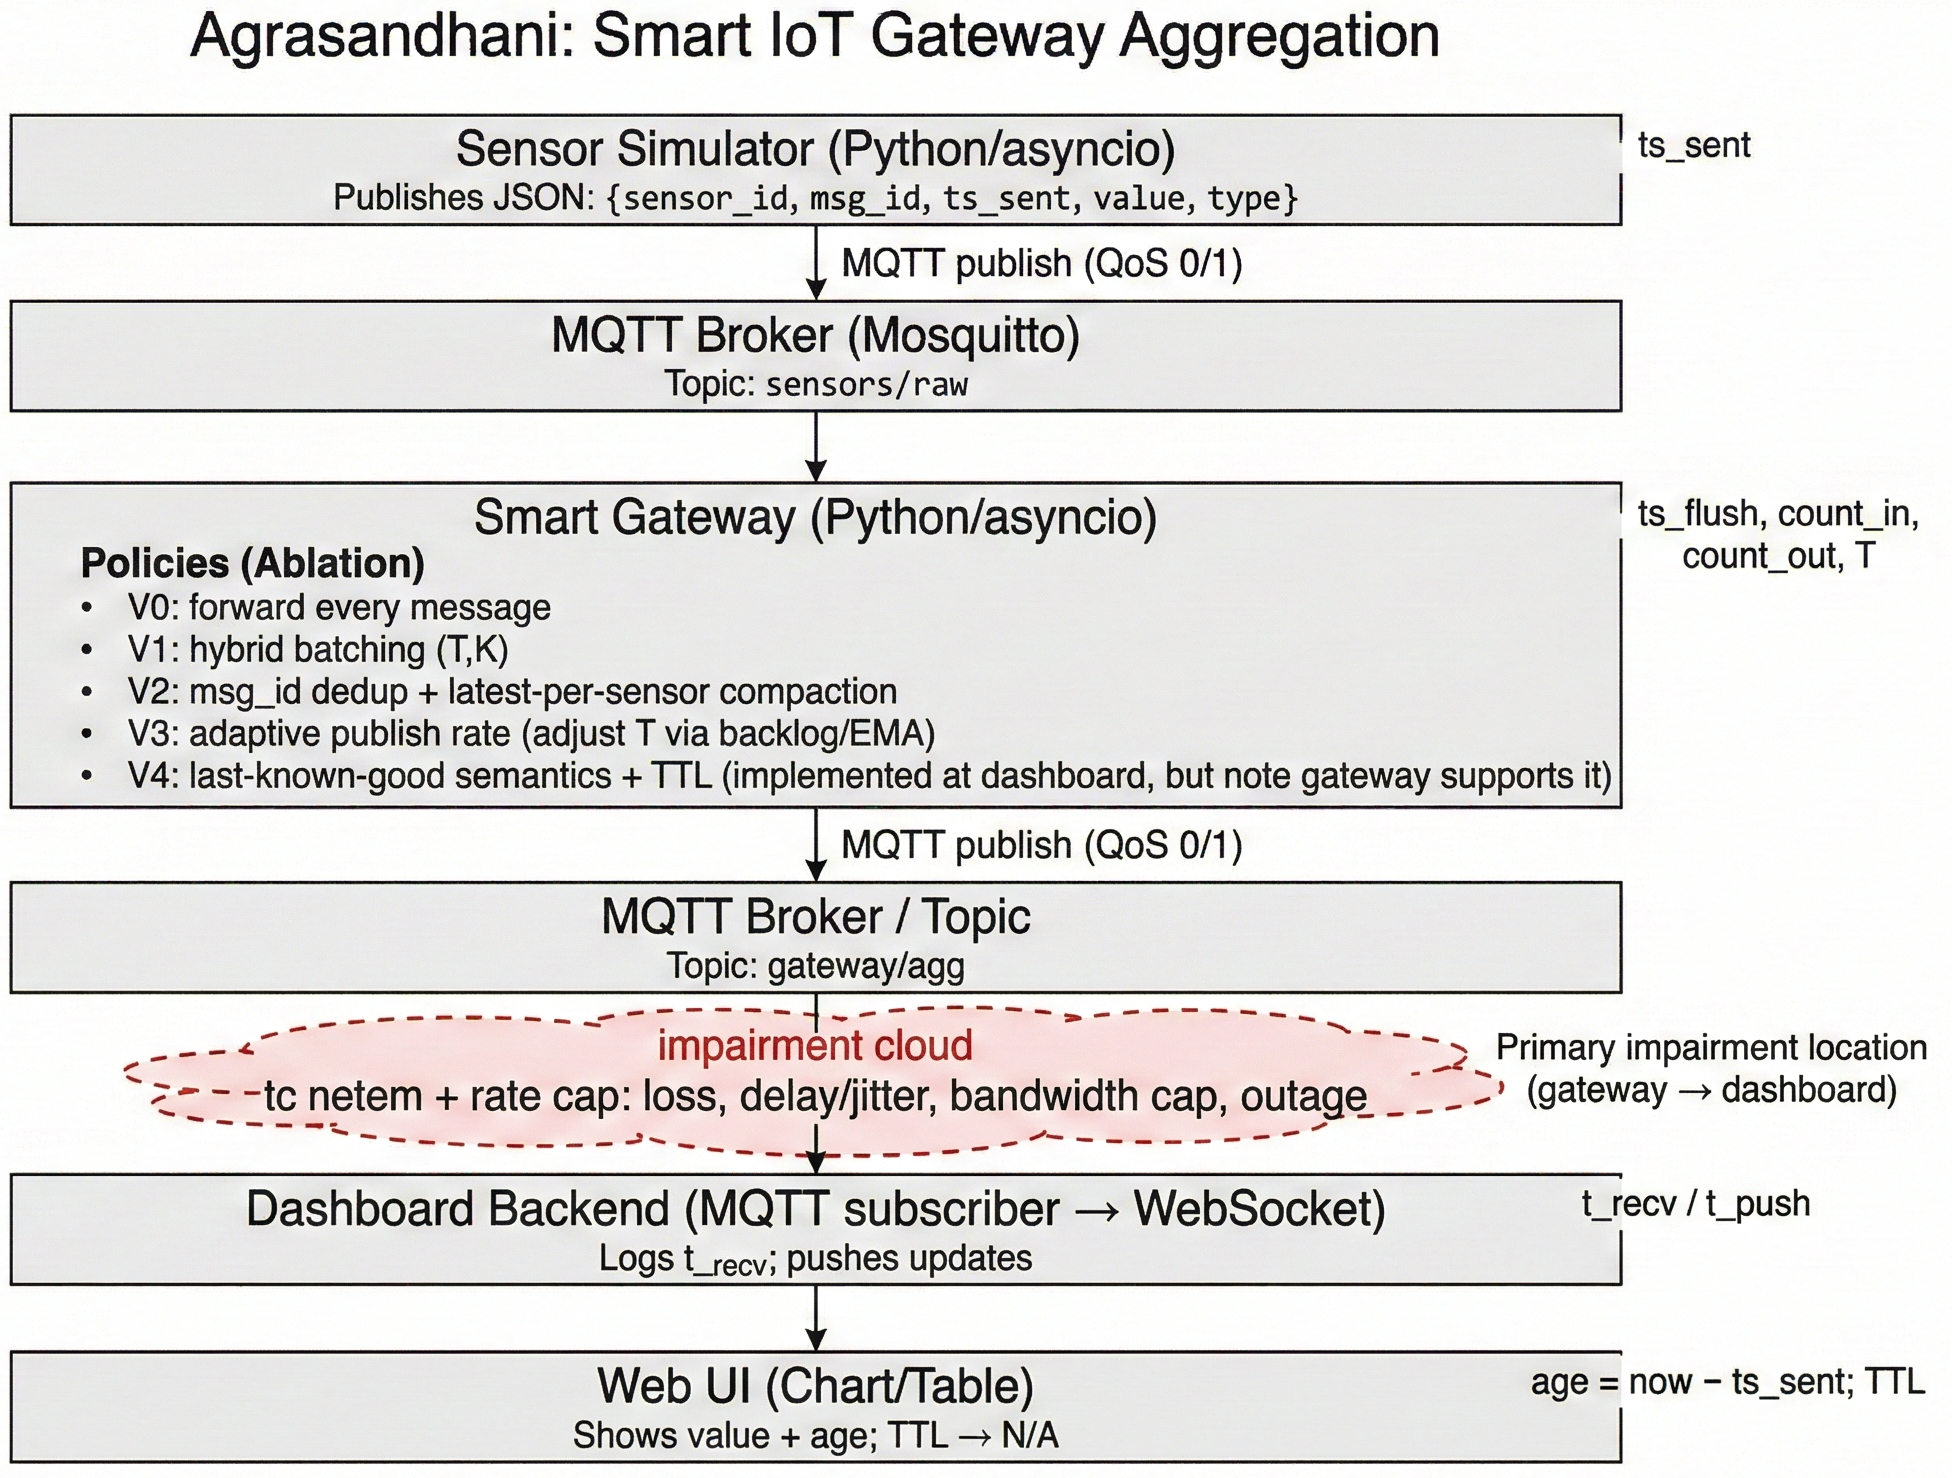
\includegraphics[width=\linewidth,height=\textheight,keepaspectratio]{Sections/approach-cs537.png}
  \caption{Agrasandhani end-to-end pipeline.}
  \label{fig:architecture}
\end{figure}

% \subsection{Approach Details}
% Describe the details of each component in this subsection

\section{Experimental Evaluation}

% [proposal] Research questions
We structure the evaluation of Agrasandhani around the following research questions (RQs), which directly reflect the failure modes of naive forwarding and the design goals of smart aggregation under MQTT and degraded networks. \textbf{RQ1 (Bandwidth vs. timeliness):} How much does hybrid batching and latest-per-sensor compaction reduce gateway-to-dashboard bandwidth compared to forwarding every message, and what latency/tail-latency cost does this introduce under normal and bursty loads? \textbf{RQ2 (Reliability-induced duplicates):} Under MQTT QoS~1 (``at least once'' delivery), which may introduce duplicate deliveries via retransmissions \cite{mqtt311}, how effective is message-ID-based deduplication at reducing duplicate-induced overhead while preserving correct state at the dashboard? \textbf{RQ3 (Robustness under impairments):} Under deterministic last-hop impairments (bandwidth caps, loss, delay, jitter, and short outages) injected with Linux traffic control (e.g., \texttt{tc netem}) \cite{jurgelionis2011_netem_empirical}, which gateway variant best maintains dashboard stability as measured by data loss, update jitter, and tail latency? \textbf{RQ4 (User-visible freshness):} How does last-known-good caching with an explicit age indicator and TTL affect the freshness distribution (age of displayed values) during and after impairments, and what trade-offs emerge between reduced communication and increased staleness? \textbf{RQ5 (Ablation and attribution):} Across an ablation ladder (V0--V4), which individual mechanism (batching, compaction, adaptive publish rate, or last-known-good semantics) accounts for the largest improvements for each metric?

\subsection{Evaluation Setting}
% [proposal] Evaluation plan
We will evaluate Agrasandhani using an end-to-end local testbed consisting of (i) a Python/asyncio sensor simulator publishing JSON messages \texttt{\{sensor\_id, msg\_id, ts\_sent, value, type\}} to an MQTT broker, (ii) a smart gateway subscribing to the raw topic and publishing aggregated updates to an output topic, and (iii) a lightweight dashboard backend that subscribes to aggregated updates and streams them to a browser UI over WebSockets. The primary comparison is an ablation ladder of gateway variants: V0 (naive forward-every-message), V1 (hybrid batching with flush every $T$ ms or $K$ messages), V2 (V1 plus two-stage deduplication and latest-per-sensor compaction), V3 (V2 plus adaptive publish rate by adjusting $T$ based on publish health signals such as send time and queue backlog), and V4 (V3 plus last-known-good dashboard semantics with explicit age and TTL). For each variant, we will run MQTT under QoS~0 and QoS~1 to expose reliability/duplicate effects; MQTT v3.1.1 defines QoS~0 as ``at most once'' and QoS~1 as ``at least once'' delivery \cite{mqtt311}. We will sweep workload intensity by varying the number of simulated sensors and their rate schedule (including deterministic burst phases), while using a mixed sensor model (slowly changing versus spiky values) to reflect heterogeneous update dynamics. To stress the user-visible last hop, we inject deterministic, repeatable degradations primarily on the gateway-to-dashboard path using the application-layer impairment proxy, with optional host-level Linux traffic control (bandwidth caps plus \texttt{tc netem} for loss, delay, jitter, and outage-like disruptions) in the same last-hop context \cite{jurgelionis2011_netem_empirical}. This placement matches the measured downstream evidence, which is collected from proxy-level frame and byte counters. Each condition will be executed for multiple trials (e.g., 2--3) with fixed random seeds to support repeatability. We will report end-to-end latency from \texttt{ts\_sent} to dashboard receipt/display (including p50/p95/p99), message rate (msgs/sec) at each stage, bandwidth usage (bytes/sec) on the gateway egress, and data loss defined via missing/late updates inferred from per-sensor \texttt{msg\_id} sequences. In addition, we will measure user-visible stability via update jitter (inter-arrival variance) and freshness via the age distribution of displayed values (with TTL-based staleness marking), enabling a rigorous characterization of the trade-offs between communication reduction, timeliness, and dashboard robustness under degraded networks.

\subsection{Evaluation Results}
All quantitative claims in this section are traceable to generated artifacts under \texttt{report/assets} and copied paper assets under \texttt{research\_paper/figures} and \texttt{research\_paper/tables}. The source runs are the final April evidence runs and their companion sweeps listed in \texttt{report/assets/evidence\_manifest.json}.

\begin{figure*}[t]
	\centering
	
\includegraphics[width=\linewidth]{figures/main_outage_frame_rate.png}
	\caption{Downstream Frame Rate Over Time During Outage: V0 vs V2 vs V4 (Intel, outage\_5s, QoS0). V0 shows bursty/high downstream frame rate, while V2 and V4 remain much lower and steadier before, during, and after outage. In this evidence set, smart variants reduce downstream frame cadence by roughly 95--97\% versus naive forwarding, stabilizing the visualization stream around outage and recovery.}
	\label{fig:main-outage-frame-rate}
\end{figure*}

\begin{table}[t]
\centering
\caption{Primary Intel summary (QoS~0, means across three replicated trials).}
\label{tab:main-summary}
\scriptsize
\setlength{\tabcolsep}{3pt}
\renewcommand{\arraystretch}{1.03}
\begin{adjustbox}{max width=\columnwidth}
\begin{tabular}{@{}lrr>{\raggedleft\arraybackslash}p{0.16\columnwidth}>{\raggedright\arraybackslash}p{0.26\columnwidth}@{}}
\toprule
Variant & Frames & Bytes & \makecell[r]{Latency p95\\(ms)} & Scenario \\
\midrule
V0 & 132 & 12069 & 31.9 & clean \\
V2 & 5 & 13051 & 276.2 & clean \\
V4 & 6 & 17641 & 607.7 & clean \\
V0 & 132 & 12069 & 121.5 & \nolinkurl{bandwidth_200kbps} \\
V2 & 5 & 13051 & 271.5 & \nolinkurl{bandwidth_200kbps} \\
V4 & 6 & 17641 & 573.7 & \nolinkurl{bandwidth_200kbps} \\
V0 & 128 & 11725 & 115.7 & \nolinkurl{loss_2pct} \\
V2 & 4 & 12129 & 267.0 & \nolinkurl{loss_2pct} \\
V4 & 5 & 16845 & 546.0 & \nolinkurl{loss_2pct} \\
V0 & 116 & 10605 & 119.8 & \nolinkurl{outage_5s} \\
V2 & 4 & 11401 & 279.1 & \nolinkurl{outage_5s} \\
V4 & 6 & 17641 & 541.7 & \nolinkurl{outage_5s} \\
\bottomrule
\end{tabular}
\end{adjustbox}
\end{table}


Figure~\ref{fig:main-outage-frame-rate} is the primary paper figure. It shows the user-visible effect of aggregation on rendering cadence under outage, where baseline V0 remains bursty and smart variants maintain a low-rate stream. The latency CDF for clean QoS0 (V0/V2/V4) is shown in \texttt{research\_paper/figures/intel\_clean\_qos0\_latency\_cdf.png}, and confirms the expected latency-versus-stability tradeoff.

Bandwidth-over-time and message-rate-over-time outage traces are provided in \texttt{research\_paper/figures/intel\_outage\_qos1\_bandwidth\_over\_time.png} and \texttt{research\_paper/figures/intel\_outage\_qos1\_message\_rate\_over\_time.png}. The batch-window tradeoff is shown in \texttt{research\_paper/figures/intel\_v2\_batch\_window\_tradeoff.png}, where larger windows increase latency and reduce frame cadence, with byte volume changing across the sweep.

The V1 vs V2 isolation result appears in \texttt{research\_paper/figures/intel\_v1\_vs\_v2\_isolation.png} and \texttt{research\_paper/tables/intel\_v1\_vs\_v2\_isolation.md}. It shows small or mixed effects beyond batching for this configuration. The adaptive V2 vs V3 impairment comparison in \texttt{research\_paper/figures/intel\_v2\_vs\_v3\_adaptive\_impairment.png} shows a null result under tested thresholds.

Freshness/retention behavior during outage is shown by the age-over-time trace \texttt{research\_paper/figures/intel\_outage\_qos0\_v0\_vs\_v4\_age\_over\_time.png} and table \texttt{research\_paper/tables/intel\_outage\_qos0\_v0\_vs\_v4\_freshness.md}. In this setup, last-known-good improves visibility/retention but not age freshness. QoS0 vs QoS1 side-by-side outcomes are shown in \texttt{research\_paper/figures/intel\_qos\_comparison.png} and \texttt{research\_paper/tables/intel\_qos\_comparison.md}, with minimal differences in this local environment.
\section{Action Plan}
\label{sec:action-plan}

We will follow an implementation-first plan with fixed internal deadlines to ensure completion and allow time for repeated experiments and analysis.

\begin{itemize}[leftmargin=*]
  \item \textbf{Week 1:} Repository + Mosquitto setup; implement sensor simulator publishing \texttt{sensors/raw}; logging skeleton (CSV/JSON).
  \item \textbf{Week 2:} Implement V0 (naive forwarder) and dashboard backend + WebSocket + minimal web UI.
  \item \textbf{Week 3:} Implement V1 (hybrid batching with $(T,K)$) and V2 (msg\_id dedup + latest-per-sensor compaction); add compression ratio metrics.
  \item \textbf{Week 4:} Implement V3 adaptive publish-rate control (control law + telemetry of $T(t)$, backlog, publish-time EMA).
  \item \textbf{Week 5:} Implement V4 dashboard semantics (age display + TTL to mark stale/N/A); add freshness metric logging.
  \item \textbf{Week 6:} Add deterministic impairment scripts for loss/delay/jitter/bandwidth cap/outage using \texttt{tc}; run initial experiment matrix.
  \item \textbf{Week 7:} Full experiment reruns (2--3 trials/condition), plot generation, threats-to-validity, write-up polish.
\end{itemize}
\section{Related Work}

Work on edge and fog data reduction consistently treats filtering, aggregation, and adaptation as lightweight mechanisms for reducing communication pressure without relocating the full analytics stack into the network. Surveys by Pioli et al.\ and Sadri et al.\ emphasize both the practical appeal of such mechanisms and the need for evaluations that report trade-offs explicitly rather than assuming universal gains \cite{pioli2022_edge_data_reduction_mapping,sadri2022_fog_data_reduction_survey}. Agrasandhani follows this line of work at the gateway layer, but evaluates the policies against dashboard-facing outcomes: downstream frame cadence, display latency, and visible age under last-hop impairment.

MQTT-specific work motivates the treatment of delivery semantics, duplicates, and freshness. The MQTT 3.1.1 specification distinguishes QoS~0 and QoS~1 delivery guarantees, and Kovalchuk et al.\ note that at-least-once delivery can require application-side handling of duplicate messages \cite{mqtt311,kovalchuk2018_mqtt_architecture_delay}. Palmese et al.\ argue for adaptation under changing network conditions, while Yates et al.\ frame freshness as an explicit observer-side property rather than a by-product of throughput \cite{palmese2022_adaptive_qos_mqttsn,yates2021_age_of_information_survey}. These ideas align with Agrasandhani's batch-window control, compaction, and age-aware dashboard semantics, even though the measured adaptive result here remains negative under the tested thresholds.

Methodologically, the paper is closer to controlled impairment studies than to open-ended deployment measurement. Jurgelionis et al.\ and Garcia and Hurtig argue that deterministic impairment is valuable because protocol and application behavior can then be compared under repeatable degradations \cite{jurgelionis2011_netem_empirical,garcia2016_kaunetem_netdev}. Agrasandhani adopts that methodological stance by using a deterministic application-layer impairment proxy on the gateway-to-dashboard path and by reporting proxy-side outputs as the canonical source of truth for dashboard-facing stability.



\bibliographystyle{ACM-Reference-Format}
\bibliography{references}

\end{document}
